\chapter{Results}
\label{ch:results}
The data gathered, cleaned and stored in the previous parts of this project is now transformed, in order to be a foundation for discovering new knowledge through the web application interface. This simple subproject was written without much giving much attention to the front-end development or any user experience whatsoever. Its purpose is to provide a user-friendly communication with the database, narrowed to the specialized queries for answering the users questions:

\begin{figure}
    \centering
    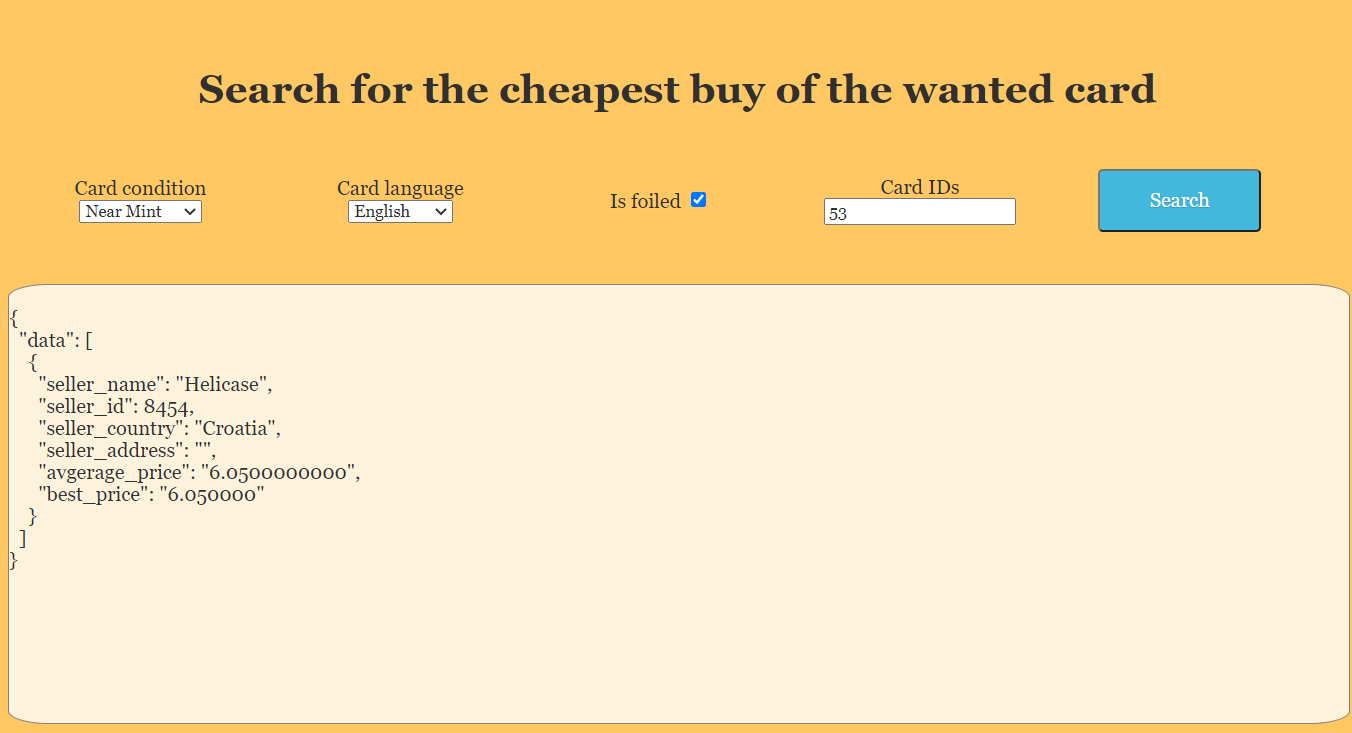
\includegraphics[width=\textwidth]{figures/cheapest_buy.png}
    \caption{Selecting sellers that sell the given card for the lowest price}
    \label{fig:cheapest_buy}
\end{figure}

\begin{figure}
    \centering
    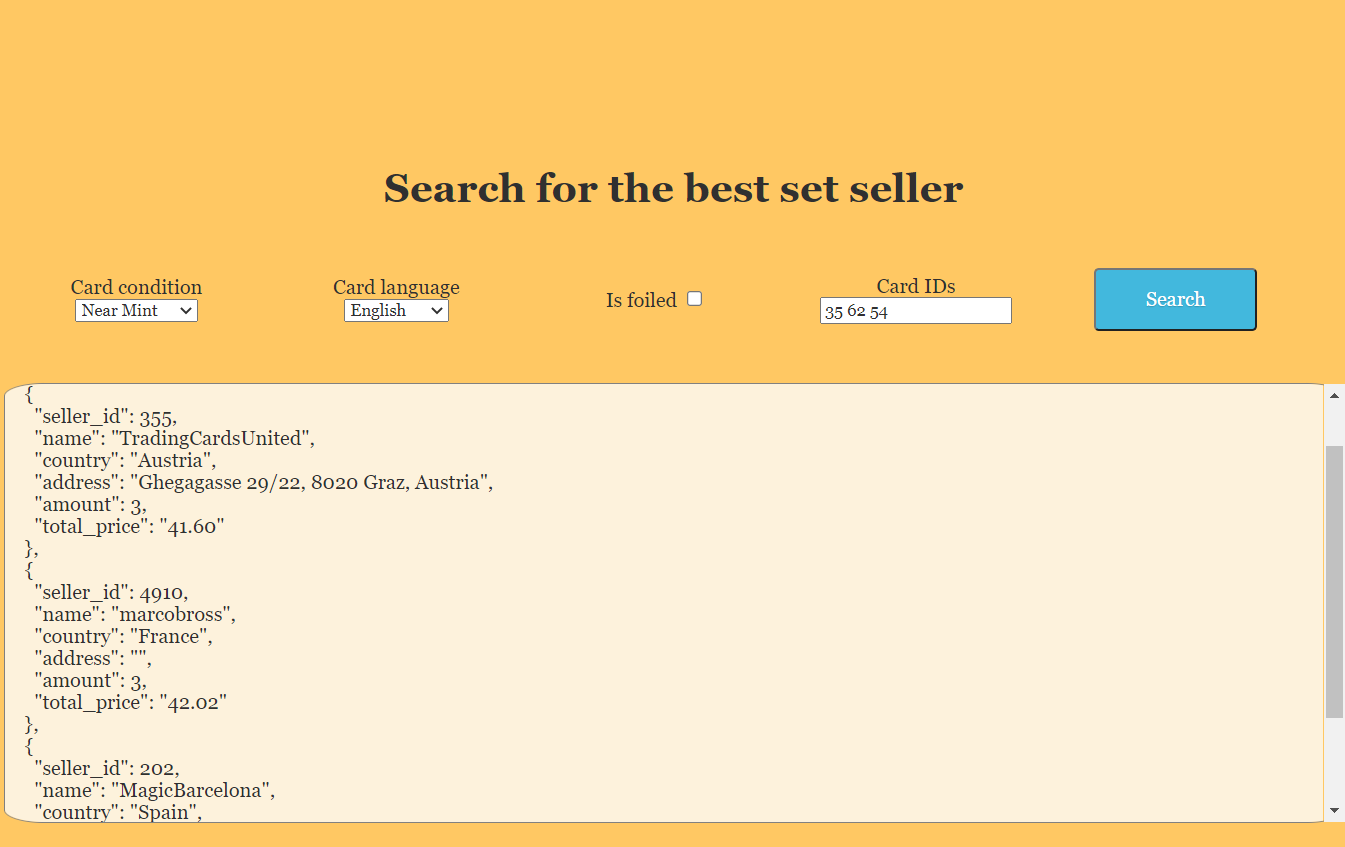
\includegraphics[width=\textwidth]{figures/best_set_seller.png}
    \caption{Finding sellers selling all three cards for the lowest total price}
    \label{fig:best_set_seller}
\end{figure}

\begin{enumerate}
    \item Cheapest Buy: targeting three sellers which sell the provided card or cards for the lowest price (Fig. \ref{fig:cheapest_buy}).
    \item Best Set Seller: finding a seller with the most provided cards on sale, ordered by the lowest sum (Fig. \ref{fig:best_set_seller}).
    \item Dealmakers: identifying those sellers, whose offers stand out as the most discounted among others (Fig. \ref{fig:dealmakers}).
    \item Deal Finder: ordering the provided cards from the highest discount available to the card with most ordrinary price (Fig. \ref{fig:deal_finder}).
\end{enumerate}

\begin{figure}
    \centering
    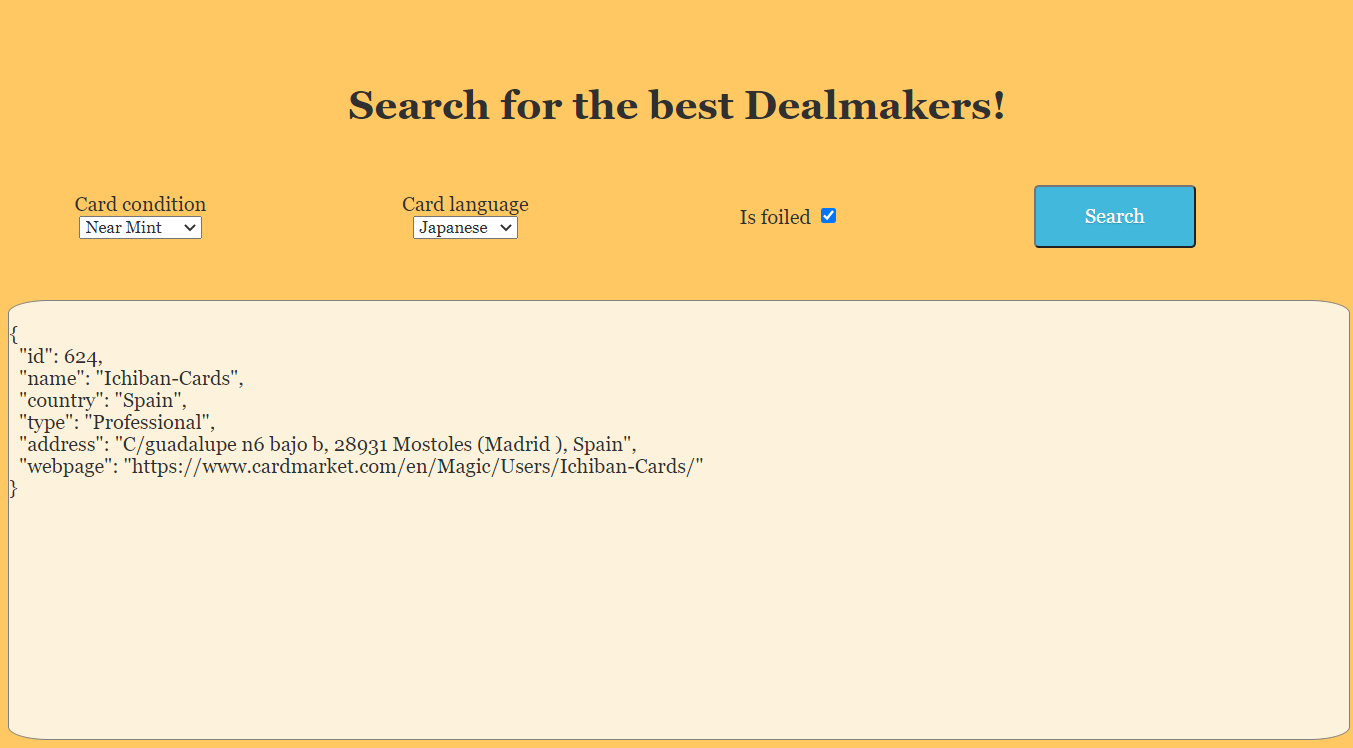
\includegraphics[width=\textwidth]{figures/dealmakers.png}
    \caption{Finding sellers with the highest discount score}
    \label{fig:dealmakers}
\end{figure}

\begin{figure}
    \centering
    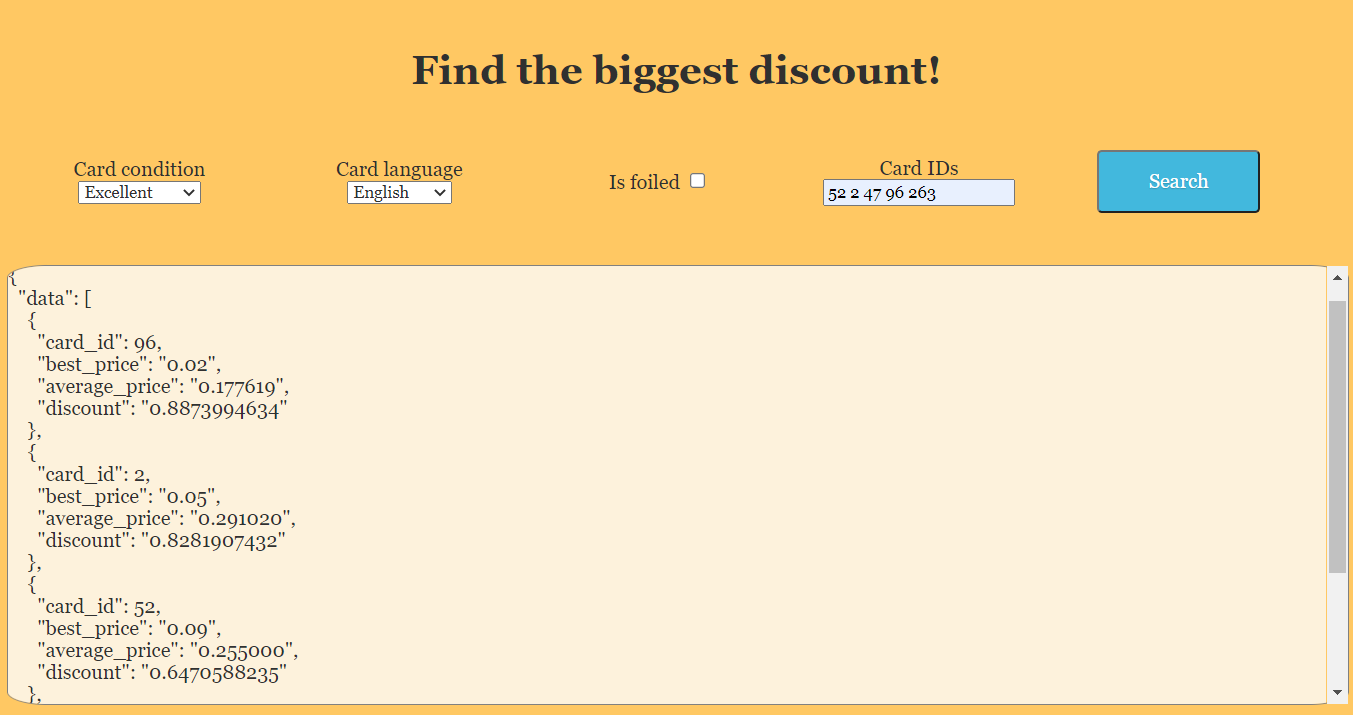
\includegraphics[width=\textwidth]{figures/deal_finder.png}
    \caption{Ordering cards by the discount available}
    \label{fig:deal_finder}
\end{figure}

\section{Data analysis}
The end results of the data analysis are plots saved in the \textit{analysis} directory. Various combinations of dataframe methods from the \textit{pandas} library are used to obtain interesting conclusions from the tables. Figure \ref{fig:available_items} shows the total number of items available for sale, registered each day since the end of September 2021. We can see a significant drop around December and January, which could be caused by the winter holidays and New Year's Eve, similar to a \textit{year-end freeze} --- a period encompassing a dozen days before and few after the end of the year, when no significant changes are made within an organization. From mid-January the number of items is back to the level from mid-December. Another chart (Fig. \ref{fig:price_chart}) presents the price statistics averaged from all cards. The moving averages (monthly and weekly) naturally have less fluctuations then the daily price. What is interesting is the observation of steady rise in value; this effect may be contributed to the economic situation related to the post-pandemic strains on various industries and a rise in inflation. The average price of all cards rised from less than \texteuro1.80 in October 2021 to over \texteuro1.95 in February 2022, which amounts to around 10\% increase over the span of five months. One can also speculate that the drop in supply around the New Year's Eve resulted in its own rise in cards' value, signified by a bump in the weekly average at the beginning of January 2022. Another example is the measure of the site's popularity, calculated via the number of new sellers per year (Fig. \ref{fig:site_popularity}). These plots would indicate that the site had its most successful years from 2017 to 2019, and sellers from before 2012 are the site's veterans. \par

\begin{figure}
    \centering
    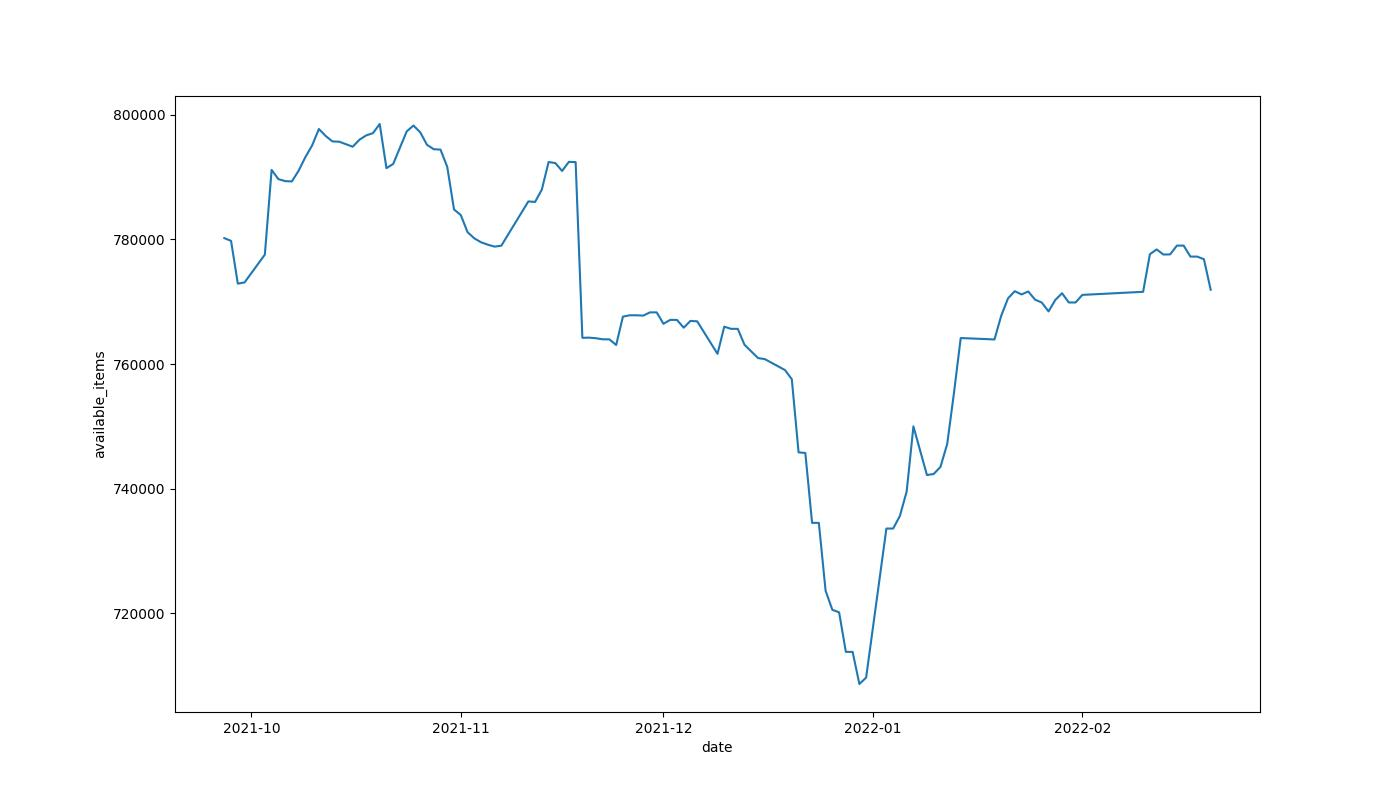
\includegraphics[width=\textwidth]{figures/available_items.jpg}
    \caption{Number of items available for sale over time}
    \label{fig:available_items}
\end{figure}

\begin{figure}
    \centering
    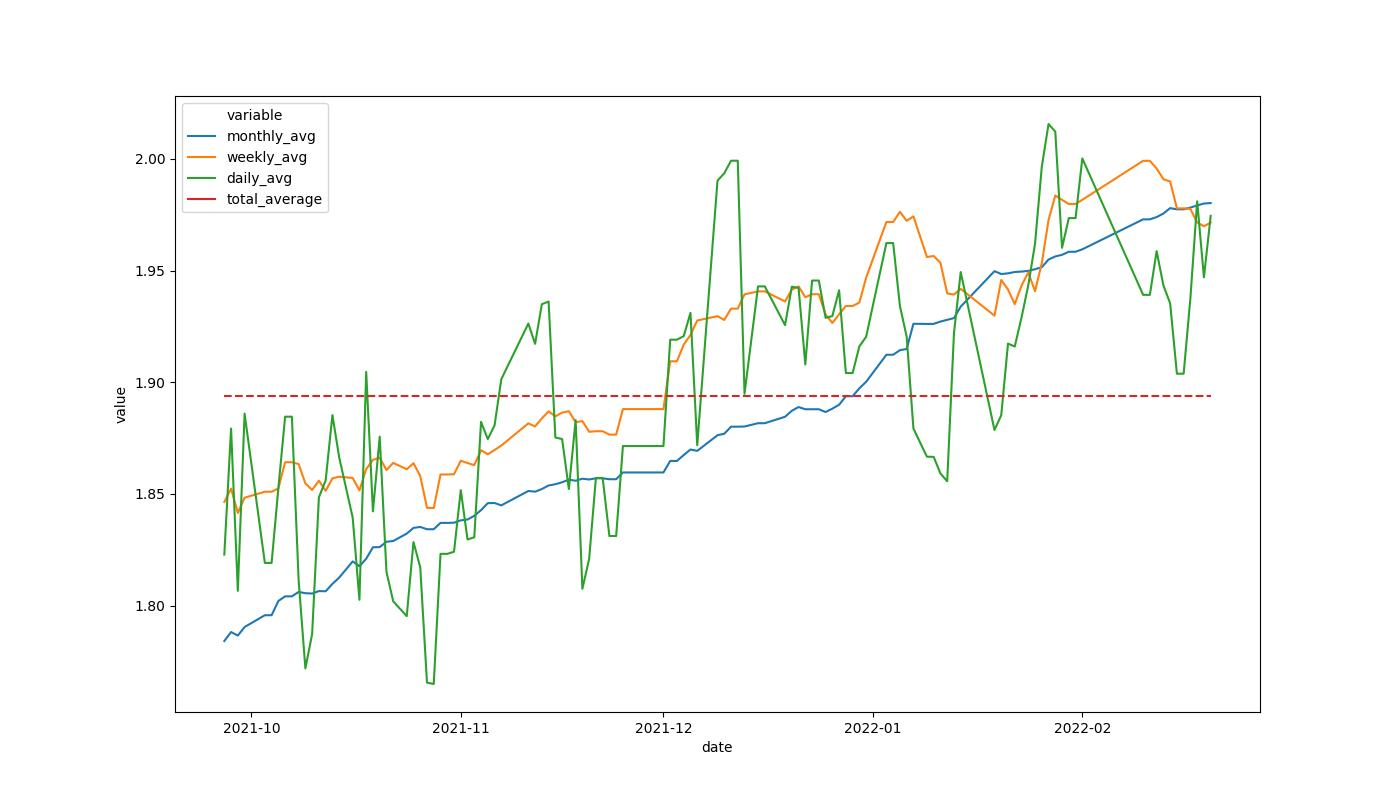
\includegraphics[width=\textwidth]{figures/price_chart.jpg}
    \caption{Price trend between October 2021 and February 2022}
    \label{fig:price_chart}
\end{figure}

\begin{figure}
    \centering
    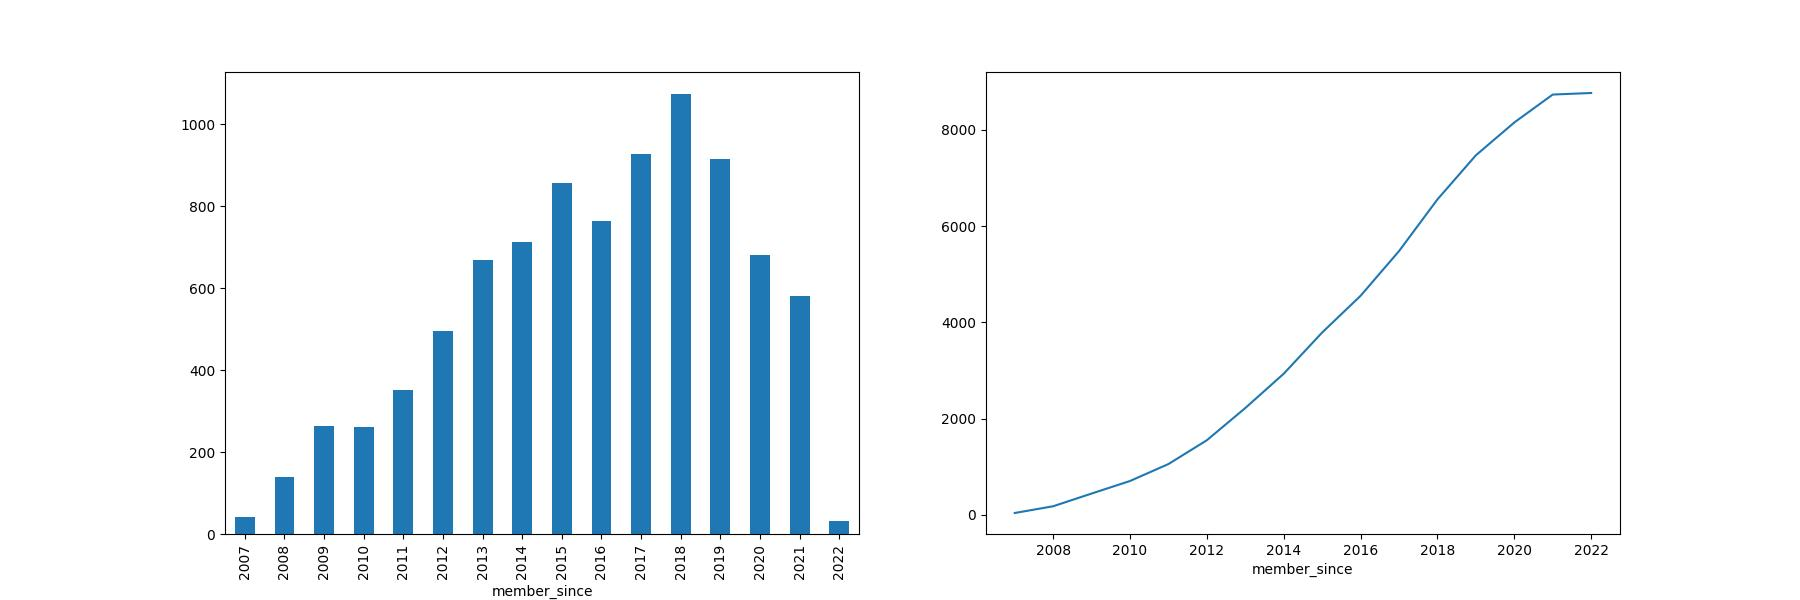
\includegraphics[width=\textwidth]{figures/site_popularity.jpg}
    \caption{Site popularity based on the number of new users per year}
    \label{fig:site_popularity}
\end{figure}

As another part of the analysis, scatterplots of best cards' prices are generated for each card individually. These help the user understand the price trends of the wanted card, by analyzing when did the top ten, thirty and fifty best deals occured, and what was the price. This way, we can provide a simple functionality for predicting the cards next \textit{good deal} without using any machine learning algorithms, but rather forcing the user's brain to intuitively continue the data into the future. For example, looking at Fig. \ref{fig:card_12} and \ref{fig:card_21} we conclude that one of the cards will probably be soon available at around \texteuro2.30, while the other is clearly rising in value and a price under \texteuro11.00 is not likely to occur anytime soon. Only the cheapest offers are taken into account, as we want to analyze the trend of the lower boundary, not the mean --- the amounts of 50, 30 and 10 were chosen with a trial-and-error approach, until the graph would become clear, information-rich, and not overwhelming. \par
More plots are available in the \textit{analysis} directory.

\begin{figure}
    \centering
    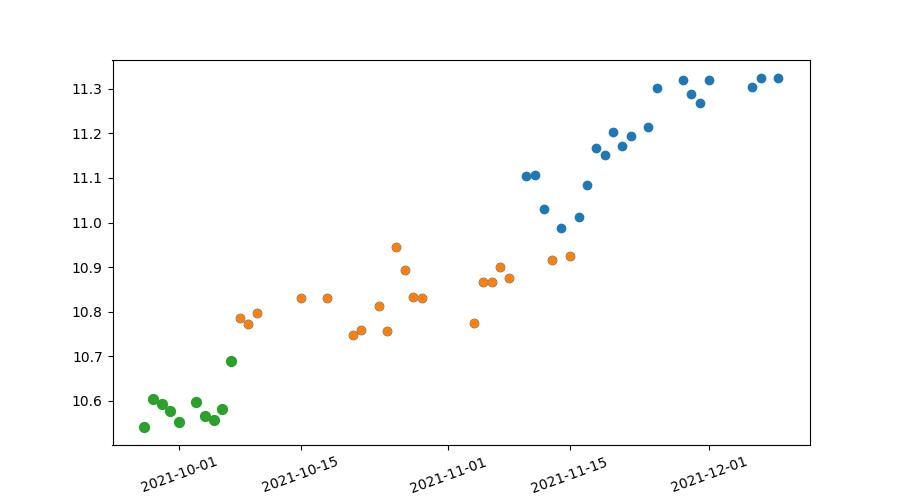
\includegraphics[width=\textwidth]{figures/card_12.jpg}
    \caption{Card 12. Best 50, 30 and 10 historical prices (blue, orange, green, respectively)}
    \label{fig:card_12}
\end{figure}

\begin{figure}
    \centering
    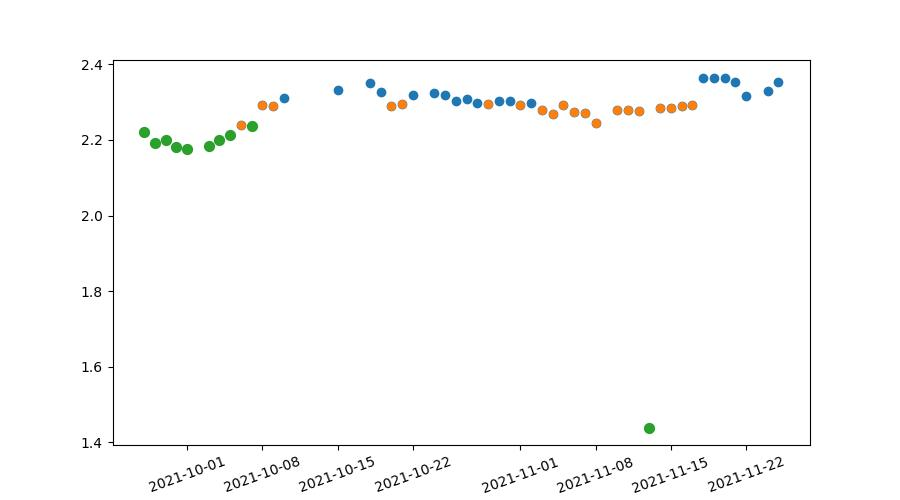
\includegraphics[width=\textwidth]{figures/card_21.jpg}
    \caption{Card 21. Best 50, 30 and 10 historical prices (blue, orange, green, respectively)}
    \label{fig:card_21}
\end{figure}

\section{Running on Fedora}
The system was successfully ran on Fedora 35 operating system, using virtualization software (\textit{Oracle VM VirtualBox 6.1.26}). After updating the system using \textit{dnf} package manager and installing \textit{docker} engine (version 20.10.12) and \textit{docker-compose}, the code was copied from private GitHub repository and executed. In Fig. \ref{fig:fedora} we can see that \textit{docker} is installed and running, which entails issuing the \texttt{docker-compose up} command will build and run the application. The proper behaviour of the system is manifested in the scenario where a complete and valid dataset has a changed checksum, because of the migration to another operating system. We can observe the containers starting in Fig. \ref{fig:fedora_init} and the discrepancy between database checksum and files checksum is detected. The database manager will halt for 15 minutes, as it waits for the data gathering module to finish its job and validate the files. Since only the checksum changed, the data is recognized to be complete and is then validated and the new checksum saved to file. As presented in Fig. \ref{fig:fedora_db_update}, during the next run we get an information that the dataset is already validated; now the dataset is validated, but not in the database, which results in an update by the manager. The data is successfully isolated, then decompressed and inserted into tables. The whole process takes about 10 minutes, and ends in saving the new checksum and cleaning up temporary local files (Fig. \ref{fig:fedora_miner}). On the same figure we see the data mining module finally getting to perform the analysis, as the database checksum is the same as the last checksum of the files. Database connection is established, helper tables are generated and the data is read and processed into charts, completing the data pipeline.

\begin{figure}[ht]
    \centering
    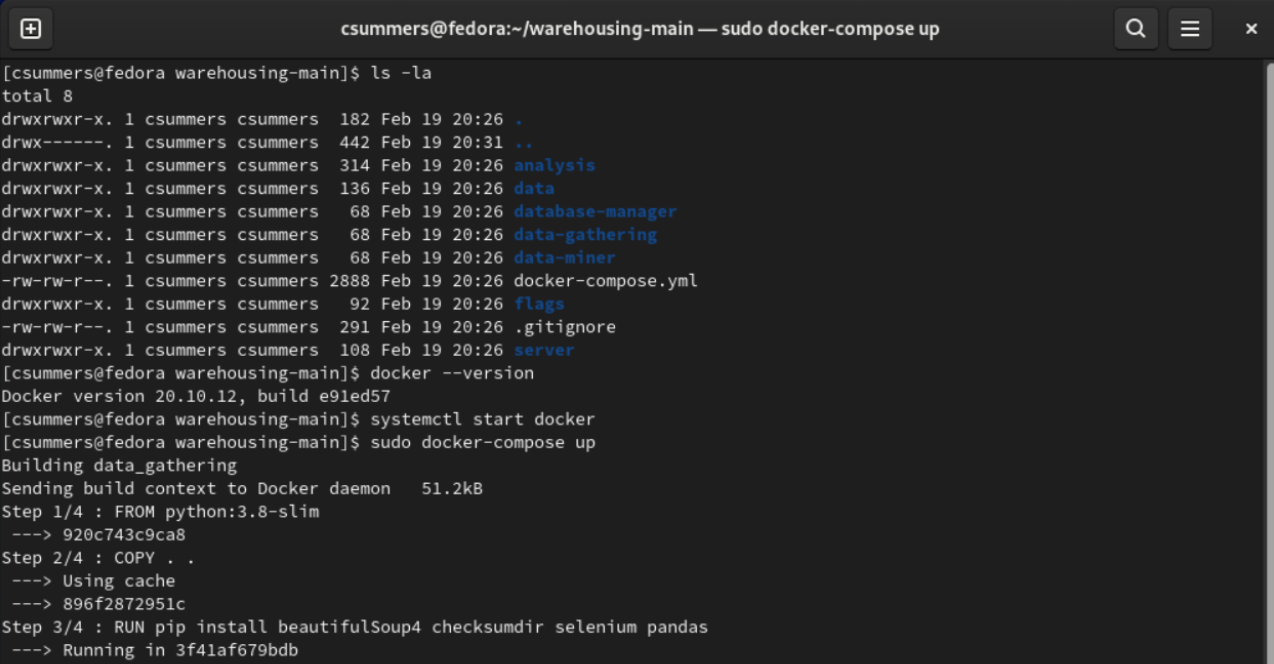
\includegraphics[width=0.9\textwidth]{figures/fedora.png}
    \caption{Fedora --- running the system}
    \label{fig:fedora}
\end{figure}

\begin{figure}
    \centering
    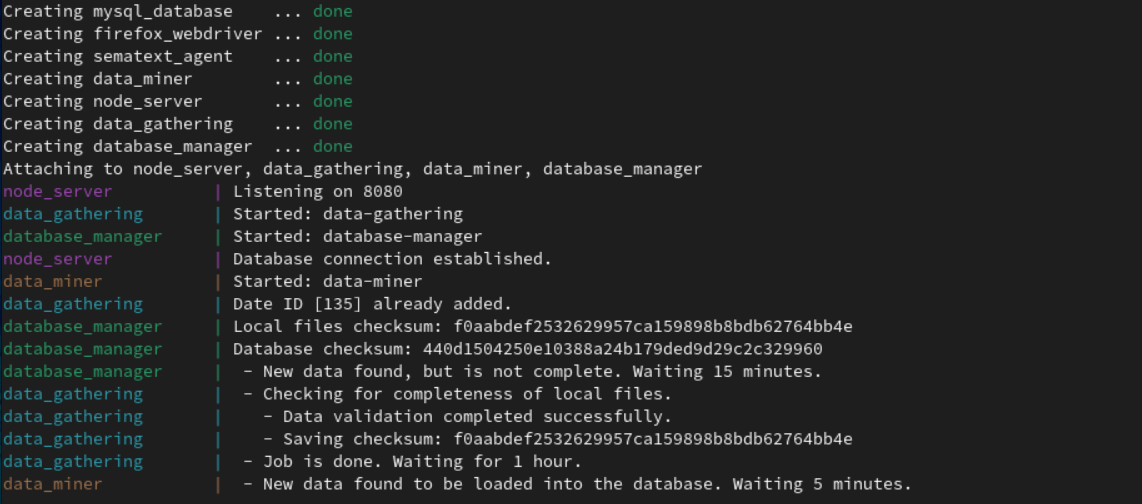
\includegraphics[width=\textwidth]{figures/fedora_init.png}
    \caption{Fedora --- containers behaviour on system init}
    \label{fig:fedora_init}
\end{figure}

\begin{figure}
    \centering
    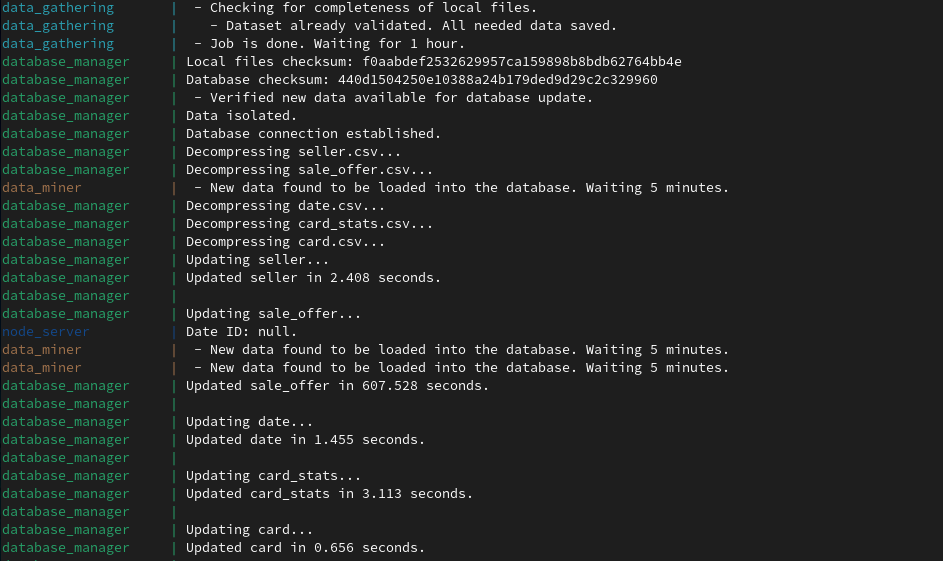
\includegraphics[width=\textwidth]{figures/fedora_db_update.png}
    \caption{Fedora --- database update}
    \label{fig:fedora_db_update}
\end{figure}

\begin{figure}
    \centering
    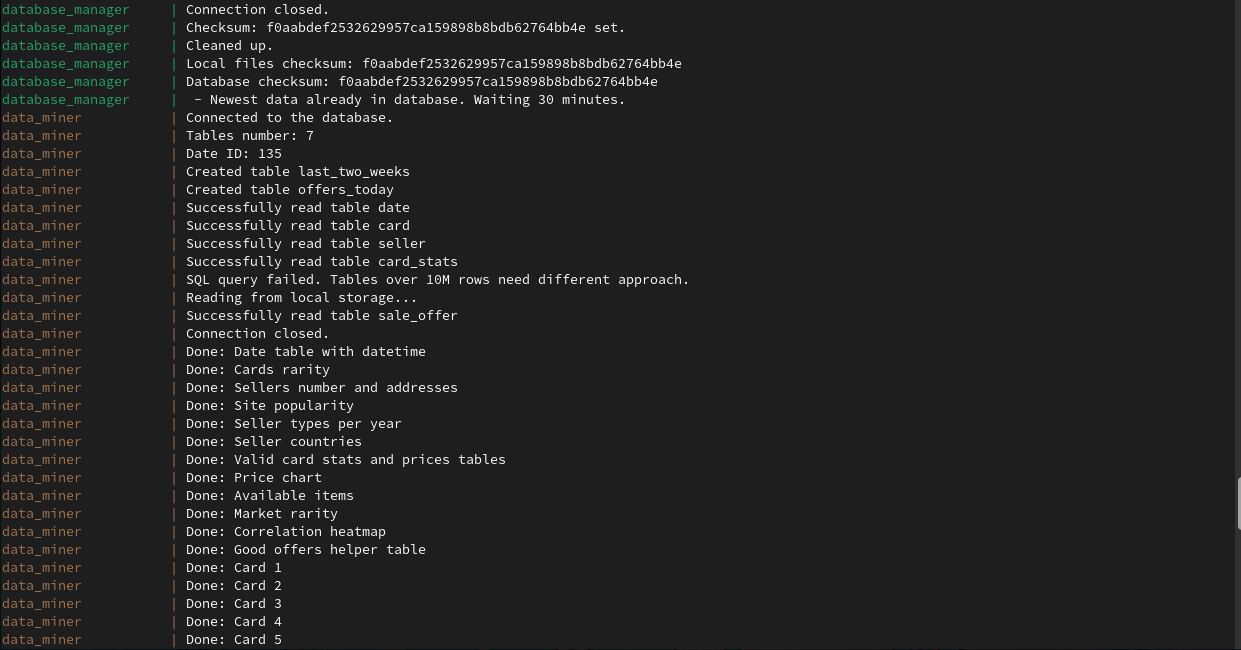
\includegraphics[width=\textwidth]{figures/fedora_miner.png}
    \caption{Fedora --- data mining and analysis}
    \label{fig:fedora_miner}
\end{figure}

Overall, the system proved to be resistant to environment changes --- given the \textit{Docker} infrastructure is available --- which is one of the main goals of containerization.

\section{Testing}
\label{s:testing}
The project was being developed without writing unit tests. Proper execution of the code was everytime assesed in conditions with some data, full data and none date. For minor changes and in initial stages, the containers were booted up separately, but with the transition to multi-container application, the internal specification of each container became dependent of the system they create with other containers (e.g. the webdriver container is visible from within the inner network, and a few elements work without the MySQL database container). All the needed testing has been done manually, but most importantly, the correctness of the results of given operation was the primary indicator of the code stability. The application was also built with the intent of running on different operating systems without problems and extensive setup. This is possible due to containerization, which provides an own microsystem for each application, isolating the core of the program from the host system. \par
The program is able to behave accordingly in unexpected conditions, as presented on Fig. \ref{fig:exception_handling}. On encountering an exception, the pickled data is first retrieved, then the container is set up to restart in 30 minutes. Another example is finding a sale offer put by a user, that hasn't been saved in the sellers table, which marks the dataset as not valid (Fig. \ref{fig:unknown_seller}).

\begin{figure}
    \centering
    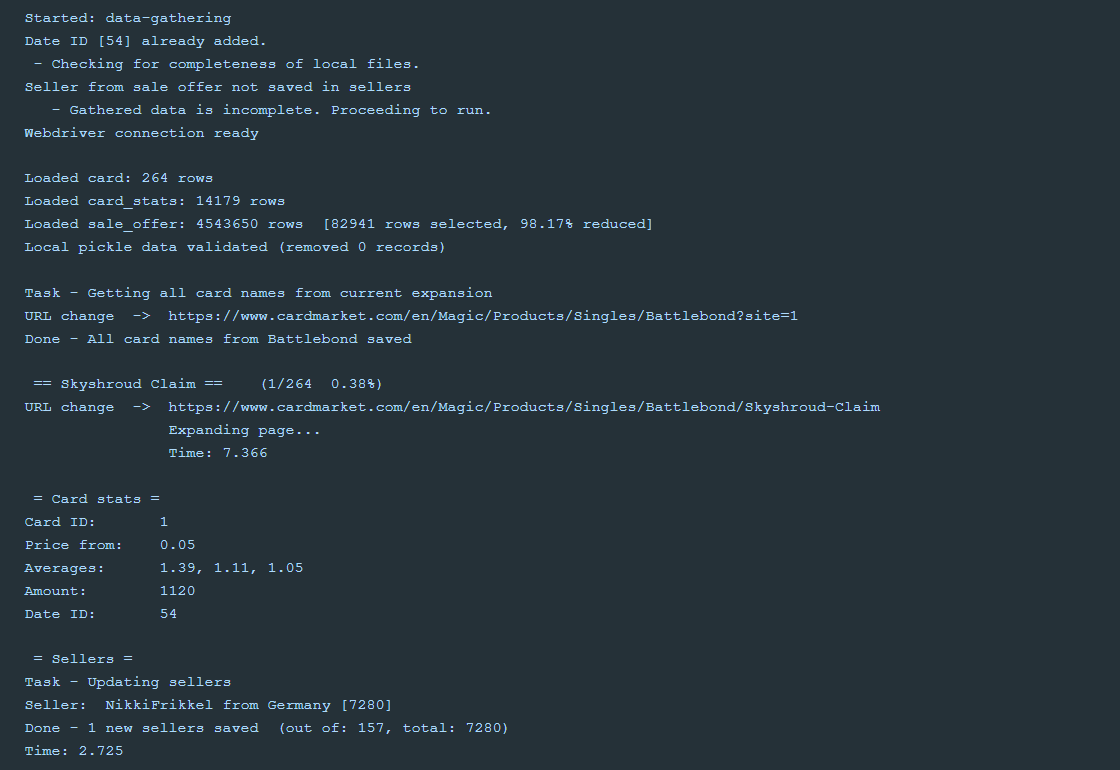
\includegraphics[width=\textwidth]{figures/unknown_seller.png}
    \caption{Handling invalid datasets --- running to complete a list of sellers wrt. sale offers}
    \label{fig:unknown_seller}
\end{figure}

\begin{figure}
    \centering
    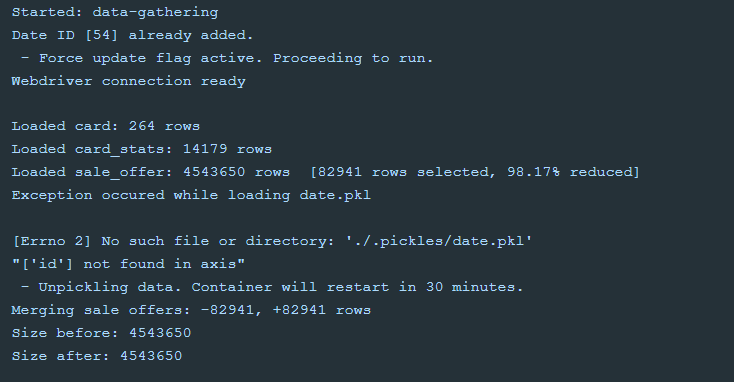
\includegraphics[width=0.875\textwidth]{figures/exception_handling.png}
    \caption{Handling an exception during the initial stages of gathering run}
    \label{fig:exception_handling}
\end{figure}


\section{Containers performance}
Using the free version of Sematext monitoring agent, the author was able to track the performance of the system, mainly the MySQL database. \par
In Fig. \ref{fig:mysql_network} we can see the amount of data received and transmitted by the database. The steady hourly level represents the data mining module, which connects to the database every 60 minutes to perform the analysis. Spikes around 1:00 am correspond to the database manager updating the tables with new data gathered from this day. \par
Fig. \ref{fig:mysql_performance} shows the load of the database. We can see the correlation between the Selects Rate and CPU and Memory load. Around 4 GB of memory are used, with additional 2--3 GB chached and buffered. \par
The last figure juxtaposes the number of tables dropped with tables created (Fig. \ref{fig:mysql_create_drop}). Due to the architecture of the system, each table is replaced by its new version, meaning every \texttt{CREATE} is paired with a \texttt{DROP}, which is reflected in the presented chart.

\begin{figure}
    \centering
    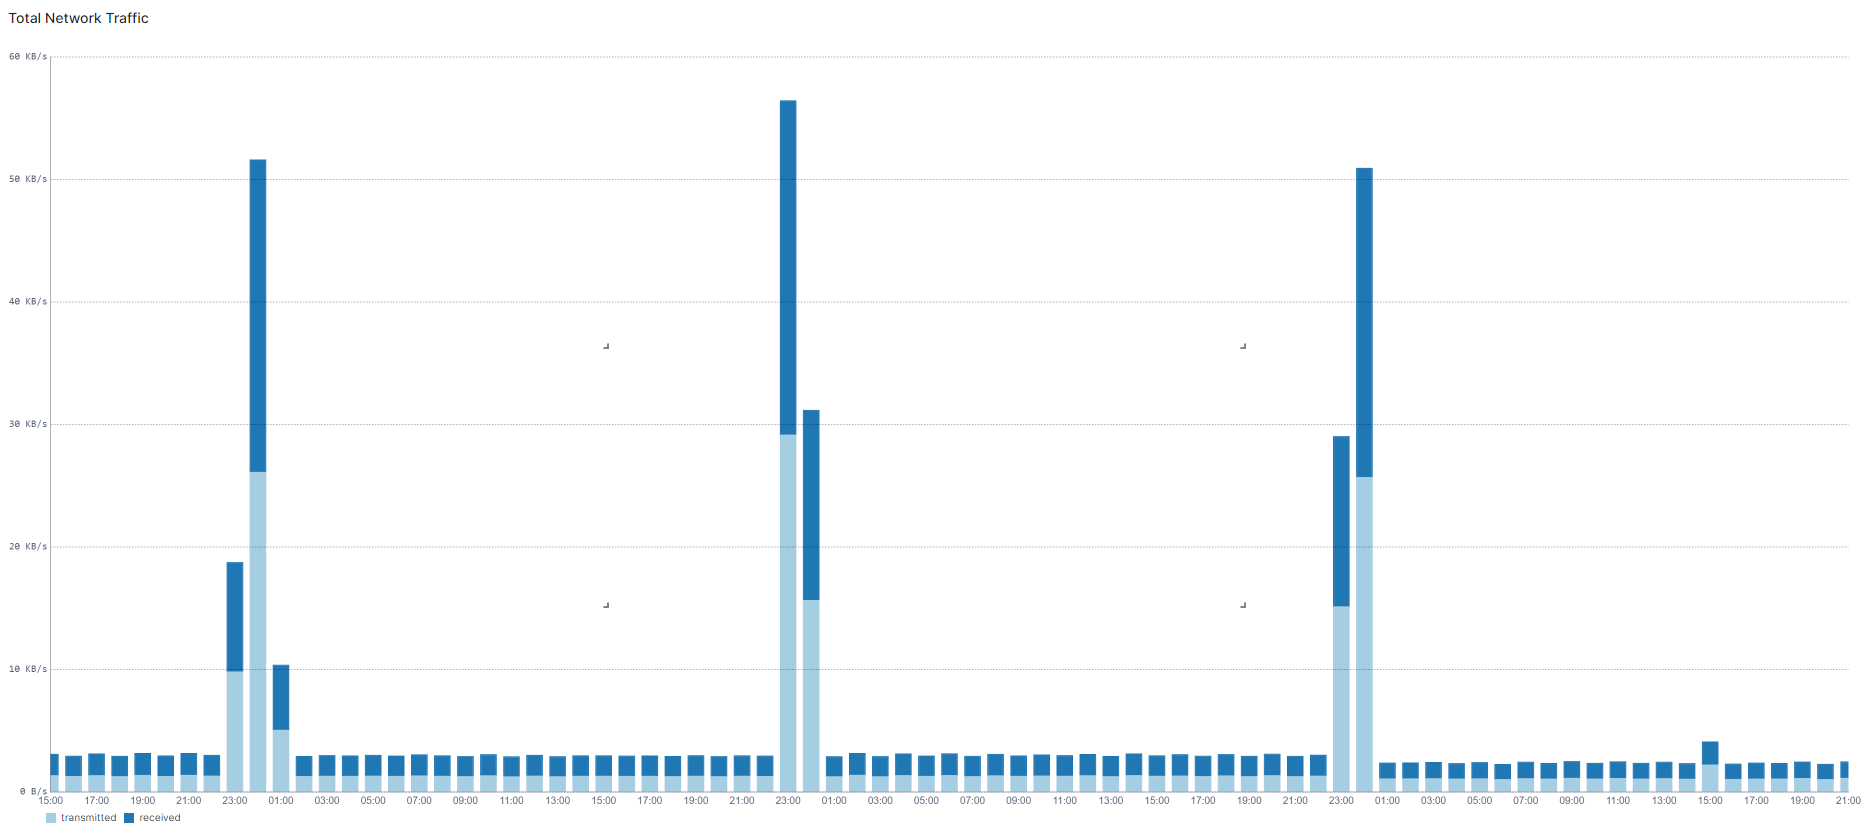
\includegraphics[width=\textwidth]{figures/mysql_network.png}
    \caption{}
    \label{fig:mysql_network}
\end{figure}

\begin{figure}
    \centering
    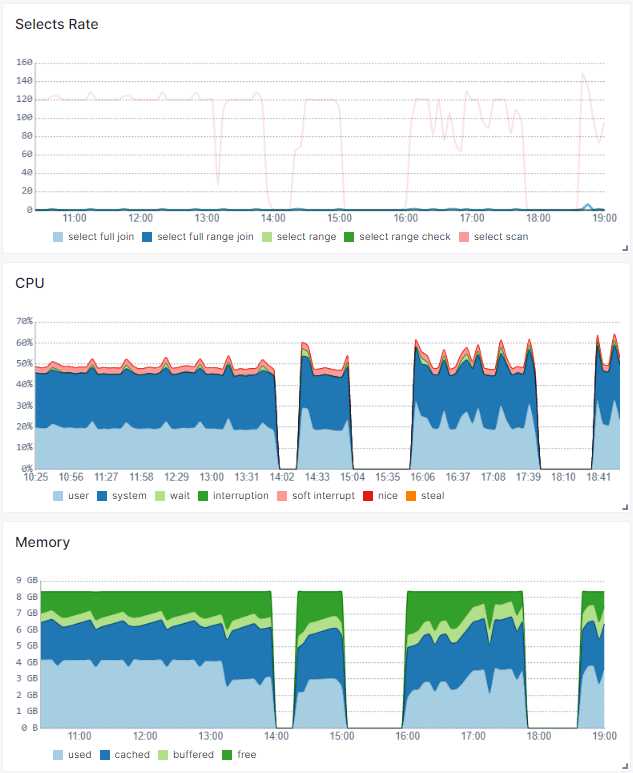
\includegraphics[width=\textwidth]{figures/mysql_performance.png}
    \caption{}
    \label{fig:mysql_performance}
\end{figure}

\begin{figure}
    \centering
    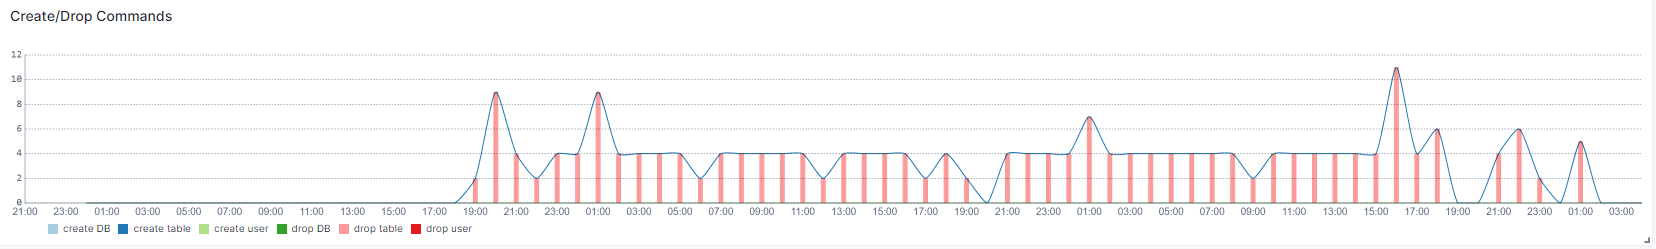
\includegraphics[width=\textwidth]{figures/mysql_create_drop.png}
    \caption{}
    \label{fig:mysql_create_drop}
\end{figure}

\section{Version control and project variation in time}
Initially, during the \textit{DWDMS} course, the project was a python program composed of several python scripts that the author and his colleagues used to gather and store the card market data. A data analysis GUI module has been implemented to showcase the possibility of utilizing the collected data. Then, the transformation of the author's part into containerized version happened, with more verbose logging. All changes were tracked using \textit{git} version control system integrated with Visual Studio Code environment. Over the span of months, the implementation of the data warehouse underwent major changes with 318 commits sent to the project. Changes in the website had to be appropriately mirrored in the gathering part of the code, time-based querying was swapped for Selenium explicit and implicit waiting methods, pickle format was added and many different SQL connection engines were tried to combat side effects of large datasets. The code was meticulously improved and polished, until the gathering time was decreased from 2.5+ hours to 1--2 hours, with most of the runs finishing in about 75 minutes. Some challenges that were faced are still to be solved, for example solving the seller dictionary fiasco when building the object iteratively and trying to save it in \textit{.pkl} format intermediately. Another issue is loading a full sale offers table into a dataframe, when it has over 10 million rows, which takes a long time and often results in a out-of-memory error. Keeping the best programming pracices in mind, all remaining encountered problems were solved, so that the system would perform its tasks and fulfill the requirements stated in sections \ref{s:functional_req} and \ref{s:nonfunctional_req}.
